%% La letra n con tilde es: 'n.

\chapter{Background}

This chapter present the fundamental concepts related to this work. The
formal definitions referring to fuzzy systems, user modeling concepts  and  gamification theory and techniques related to this method.
%--------------------------------------------------------------
%Agregue la seccion de logica difusa del articulo que me mando.
\section{User Modeling}

%%\subsection{Traditional Production Systems}

User modeling can be represented as the technique of building a model of the
user to personalize a system. The user model is commonly created as the user is
working with the system. An example is an educational application that teaches
students an individual skill: given the rules and knowledge in the user model,
the difficulty level of the exercises in the form is altered as the user
progresses.   Formally definition of user modeling according to McTear \cite{mctear1993user} : " user modeling is the process of gathering information about the users of
a computer system and of using the information to provide services or
information adapted to the specific requirements of individual users (or groups
of users)". The purpose of the user model is to have a module containing the
operations that are needed to personalize the system, and the user profile,
which includes the personal data of the user \cite{}( Mohamad et al., 2013).    System
personalization over user modeling is related to the research field of adaptive
systems; this subject is beyond the scope of this research work. Focus on the
human user, user modeling is a very cross-disciplinary research topic,
comprehending the domains of artificial intelligence, computer science, and
social science. Ideas have been co‐opted from an extensive range of subdomains,
such as human–computer interaction, e‐learning, information science, social
computing, machine learning, data mining, cognitive science, and so on \cite{kay2012coming}
\cite{kobsa2001generic}. There is interest in user modeling from both a
scientific and commercial perspective \cite{razmerita2009user}.

\subsection{Application Domains for user modeling}

Amount Research and implementation exist in this domain in which personalization
and user modeling plays an important role. This section presents several works
of these domains. To understand this topic, the different objects are divided
into three general categories:
\begin{itemize}
\item {supporting a user during a task. }
\item {giving a user a specific personalized experience. }
\item {training and educating a user.}
\end{itemize} 
The categories especially differ in the kind of user data that is used. For each
domain, the general purpose of the domain and the more accurate purpose of the
user model are discussed.

\subsection{User models for providing task support}

Task support systems are f systems that help a user during a task by either
supporting the user perform the task or by completely taking over this task
\cite{brun2010compass}(Nurmi et al., 2007). For instance,  an application that
automatically categorizes the incoming emails of the user. The goal of the user
model in these requests is to promote the efficiency of interactions with the
user, to simplify these interactions and to make complex systems more usable
\cite{razmerita2009user}\cite{fischer2001user}.
To perform this personalization, data is
collected through observations of the user. This information is related to the
user’s goals and needs, but especially to the task that the user currently is
accomplished, like the user’s task knowledge and background. Much research has
been done in this domain, but because many separate research projects are
focusing on an exact task or subject \cite{}(Sannes, 2011), it is hard to make
generalizations or to establish one delimited investigation topic. Commonly
discussed research subjects are Decision Support Systems,  Adaptive Hypermedia,
and Adaptive Ubiquitous Systems, each having his or her own specific domain and
way of personalization.  

\subsection{Decision support systems}

Decision support systems are systems that support a user with making a decision
in a complex, professional environment \cite{} (Nurmi et al., 2007). For example,  a
system used at a pharmacy for automatically checking valid combinations of
medicine. The method can be used to help the pharmacist in prescribing the right
combinations and to give information for making a decision when a problem
occurs.  The purpose of the user model in decision support systems is to present
the user with the right and appropriate information, giving different feedback
or applying various decision steps according to the characteristics of the
user.The data that is used is often associated with the user’s task and
background knowledge.    The adaptation takes place by adapting the amount and
the content of the feedback provided by the system.


Decision support systems are traditionally ruled ‐ or logic-based systems, in
which all the relevant information is represented in a knowledge base. This
means that the content of the user model itself is also highly dependent on the
way the rules and knowledge are represented.


\subsection{Adaptive Hypermedia}

Adaptive hypermedia system is a system that grant users to browse freely information
network,  structured by nodes and links, to retrieve items of information \cite{deepa2012adaptive}. For instance an internet website application.
The goal of the user model is to make the interface and structure of the system
dynamic. This enables the application to adapt to the user and to make it easier
for the user to search for and retrieve relevant information.  The data used in
the user model is related to the user’s abilities, knowledge, and goals in the
application. The adaptation happens by adjusting the structure and the
presentation style to the expected needs of the user. For example, by enhancing
web search: promoting pages that might better correspond to the user’s
characteristics, on the other hand by giving navigation support, through
highlighting certain components of a page \cite{razmerita2012user}.

\subsection{Adaptive ubiquitous systems}

Ubiquitous systems are concerned with data handling applications integrated into
everyday objects and activities (Nurmi et al., 2007).  For example the smart
energy meter, recording the energy usage in a household through small devices
distributed in a house, supporting the user with managing this energy
usage \cite{hargreaves2010making}.   
The main purpose of the user model is to
improve the system, facilitate the user’s preferences and thus make the overall
use easier.
Because the personalization can take place in every situation
and location, the data is focused on the user state and context. For example to
enable the contextualization to a current environmental change. 
The adaptation takes place by changing the behavior of, and the feedback given by the whole
system. These objects can be inferred by looking at the properties of the
objects in the user profile, or by looking at the objects in other user profiles
that are similar to the user \cite{kobsa2001generic} \cite{kay2012coming}. Because of the
predominantly commercial goal of these systems, the adaptations often take place
in a very intrusive way, to make sure the user notices the change.
Most recommender systems used on the Internet, which means that some typical
technical difficulties are associated with these kinds of user models. First,
the user profile is often only saved during the user’s visit,  which means that
fast and efficient adaption is necessary. Recommender systems often become more
precise when the user spends more time on the system. Second, the system’s
structure is often split up in a client and on a server side, where the client
side solely gathers user information and sends it to the server, where the
actual computation takes place.

\subsection{User models for providing a personal experience.}

User models for providing the user with a personal experience have the goal to
improve the user experience while using the system.  This kind of user modeling
is especially focused on more commercial fields, such as e-commerce, marketing,
and computer games, and became popular with the rise of the Internet.  The
information that is used by the user in this main domain is mostly focused on
the information that defines the user, such as the user’s preferences and
interests. Since this data is regularly delicate, privacy is a  big issue \cite{toch2012personalization}. While in other domains the privacy of the user data is also
important, in this area it is even a greater topic of discussion because the
incentive of the application developers is frequently contradictory to the
incentive of the actual user, considering gaining and sharing the user´s
personal information. For instance, user profiles are often shared among diverse
components of the same application, or even with different applications \cite{brun2010compass} \cite{karam2012modeling}, which presents additional weaknesses and
possible undesirable information sharing.  Ensuring personal data is not open to
all people, in addition to defining strict privacy policies, is thus essential
in these user models. Some investigation in this domain are.

\subsection{Recommender Systems and User Adaptive Computer Games.}

Recommender systems are concerned with presenting the user with relevant
information and suggestions. They are commonly used on the Internet, for example
on websites such as Facebook, to provide the user with personalized news,
targeted advertisements and possibly new friends \cite{brun2010compass}. The
purpose of the user model is to give the system with information that is assumed
to be important for the user. The information that is stored for this goal is
associated with the preferences of the user to certain objects, like products,
music or people. To benefit a classification of these objects, the interaction
history of the user is stored, or the user is explicitly asked to rate certain
objects. The content of the system is eventually adjusted by showing the
recently inferred objects. In these senses, objects can be inferred by looking
at the attributes of the objects in the user profile, or by looking at the
objects in other user profiles that are related to the user \cite{kobsa2001generic} 
\cite{kay2012coming}.  As a result of the predominantly commercial target of these
systems, the adaptations often take place in a very invasive way, to make sure
the user notices the change. Most recommender systems are based on the Internet,
which means that some typical technical difficulties  are associated with these
kinds of user models. First, the user profile is often only stored while the
user’s visit,  which means that fast and efficient adaption is important.
Recommender systems usually become more precise  when the user spends more time
with the system. Second, the system’s architecture is usually client-server,
where the client side gathers user information and sends it to the server, where
the  actual process takes place.

\subsection{User Adaptive Computer Games.}  

User Adaptive computer games are games that focus on increasing the perceived
value by providing a strongly individualized experience (Brisson, 2012).  For
example is a first‐person shooter that adapts the performance of the enemy
according to the shooting accuracy of the player.

The fundamental idea of the user model is to identify or classify the user, so
the appropriate adjustment is made in the computer game. The information that is
used addresses the preferences and progress of the user, such as the user´s
current  difficulty level or even the employed strategy. This data is usually
obtained through the interactions of  the user with the game, and therefor first
should be translated and formalized  before it can be  used to interpret
conclusions on a higher level. The adaptation that takes place in the game
concerns changing the content and role of the  game, such as the game
difficulty, the behavior of non‐player characters  or even the background  music
\cite{bakkes2012personalised}.

Because of the emphasis on the user, user adaptive computer games have
relatively a lot of processing power available  for personalization. In this
sense the user adaptive computer games domain is a very interesting research
domain.


\subsection{User models for educational purposes.}

Educational systems are systems developed with a teaching reason. They are
commonly applied in e‐learning,  where electronic media and Information
technologies are used for education. However, in most educational systems,  user
modeling and adaptation plays a minor role. Content is presented, and only
simple things such as the student’s progress in the course are registered. By
adding personalization to these applications, the learning value can notably
increase, ensuring that every learner achieves and reaches the highest standards
possible \cite{heller2006competence}. Also, the experience of the teacher or
supervisor can be increased through personalization, for instance through
inferring and employing the preferred teaching style. However, here we consider
the student as the user to which the system will be personalized. Thus, it is
preferable that the data stored in the user profile be interpretable by humans.
When looking at the time of adjustment in educational systems, we can make a
clear difference between adaptation while the student is doing an exercise,
which we will refer to as online adaptation, and adaptation that takes place
afterward, which we will refer to as offline adaptation. The most important
investigation domains that do utilize considerable user modeling constructions
are Intelligent  Tutoring Systems and Adaptive Educational Games.

\subsection{Intelligent Tutoring Systems.}

Intelligent Tutoring Systems (ITS) are systems that provide students automated
step‐by‐step instruction as the students complete training tasks and/or work on
exercises. An ITS has the purpose to complement or even replace the human
teacher. For example a system for teaching students how to program, with the
ability to automatically detect common mistakes \cite{elsom1993student}.

The particular goal of the user model is to select educational activities and
strategies and in addition  delivered individual feedback that is most relevant
to the user’s level of knowledge \cite{kobsa2001generic} \cite{mctear1993user}. The user
information that is stored for this purpose is the student’s state, knowledge
and level of  achievement. This data is exclusively observed over the actions
and results of the student, such as the answers the student gives. After
observing this information, it is used to infer higher level  properties, such
as the student´s learning style and other preferences.

Traditionally, just like decision support systems, information technology
systems are knowledge based systems, using formalized domain  knowledge and
rules to drive the user adjustment (adaptation). For instance stereotypes are
widely used in information technology systems \cite{kay2012coming} and represent a set of
default attributes that often co‐occur in users or in a certain group of people.
The different stereotypes that have been build differ in granularity of detail
and complexity.


\subsection{Adaptive Educational Games.} 

Adaptive Educational Games (AEGs) are complicated educational games that combine
ideas from several investigations areas, to increase the student’s learning
experience \cite{peeters2012situated}. These are especially based on  serious
games: computer games with an educational approach, where things are taught to
students by using a  playful idea \cite{korteling2011transfer} \cite{johnson2005serious}. For instance an AEG is a training application  for fire fighters, letting
the fire fighters train their skills and knowledge in a safe on a virtual
environment.
  
The objective of the user model in an AEGs is to optimize the learning process
and outcome.   The user information is considered with the advance and knowledge
of the student, but also with the  student’s mental and cognitive
characteristics. The gained data can be used to adjust the content,
presentation, and system behavior to the  student’s need, for example, by
adjusting the content, tone, or amount of presented feedback. Adaptive computer
games have a lot of processing power available for personalization,  making a
complex and interesting domain for user modeling.

\subsection{Methods for user modeling.} 

In the user modeling topic, researchers have proposed more general design
methods and frameworks to guide the developers in the process of user modeling.
These general methods are useful in research projects, where the knowledge can
be reused to adjust the user model to the system’s characteristics. Also in
commercial applications,  these general methods have proven to be useful 
\cite{brun2010compass} , because they make it easier and more feasible to implement
personalization into a system. In early work, the process of user modeling was
mostly based on the intuition and experience of the developer or researcher. In
recent work, the techniques of user modeling were essentially based on the
intuition and expertise of the developer or researcher. As the user modeling
research field evolved, there has been put much effort in creating a general way
for designing and constructing a user model, by basing decisions on more
empirical grounds and by defining methods applicable to the whole field 
\cite{kobsa2001generic} \cite{durrani1997cognitive}.

Frameworks,  methodologies, and architectures have been developed, defining the
strict process, restrictions and choices on how to design and build a user
model.  In the early days of user modeling, the focus was put on developing one
method applicable to the user modeling field as a whole. However, user modeling
is a very cross‐disciplinary research subject. Therefore, throughout the
decades, the user modeling area of research has been influenced by the important
research topics and trends of their time. For example, when information
technologies became a major subject in the early nineties, user modeling methods
were also mostly focused on the application of stereotypes, knowledge bases, and
logic to define a user model. With the rise of the Internet, the objectives of
the user modeling field change to Web-oriented applications and all the specific
problems that arise with this. Thus this connection,  also the general user
modeling methods that were developed, were focused on the popular research
domains of their time \cite{kay2012coming}. The main approaches to user modeling
did not change, but the specific filling‐in of the user model, such as which
technology to apply, did change. In this sense development of user modeling as a
whole, most researchers eventually agreed that one method to solve all problems
is not possible \cite{mctear1993user} \cite{kobsa2001generic}. Instead, a broad range of  generic
user modeling methods has been developed \cite{fischer2001user}; each of which supports
only a few of the very different manifestations of personalization. 







\section{Interactive Evolutionary Computation.}
\begin{figure*}
\captionsetup{justification=centering,margin=2cm}
\centering
\setlength\fboxsep{0pt}
\setlength\fboxrule{0.7pt}
\fbox{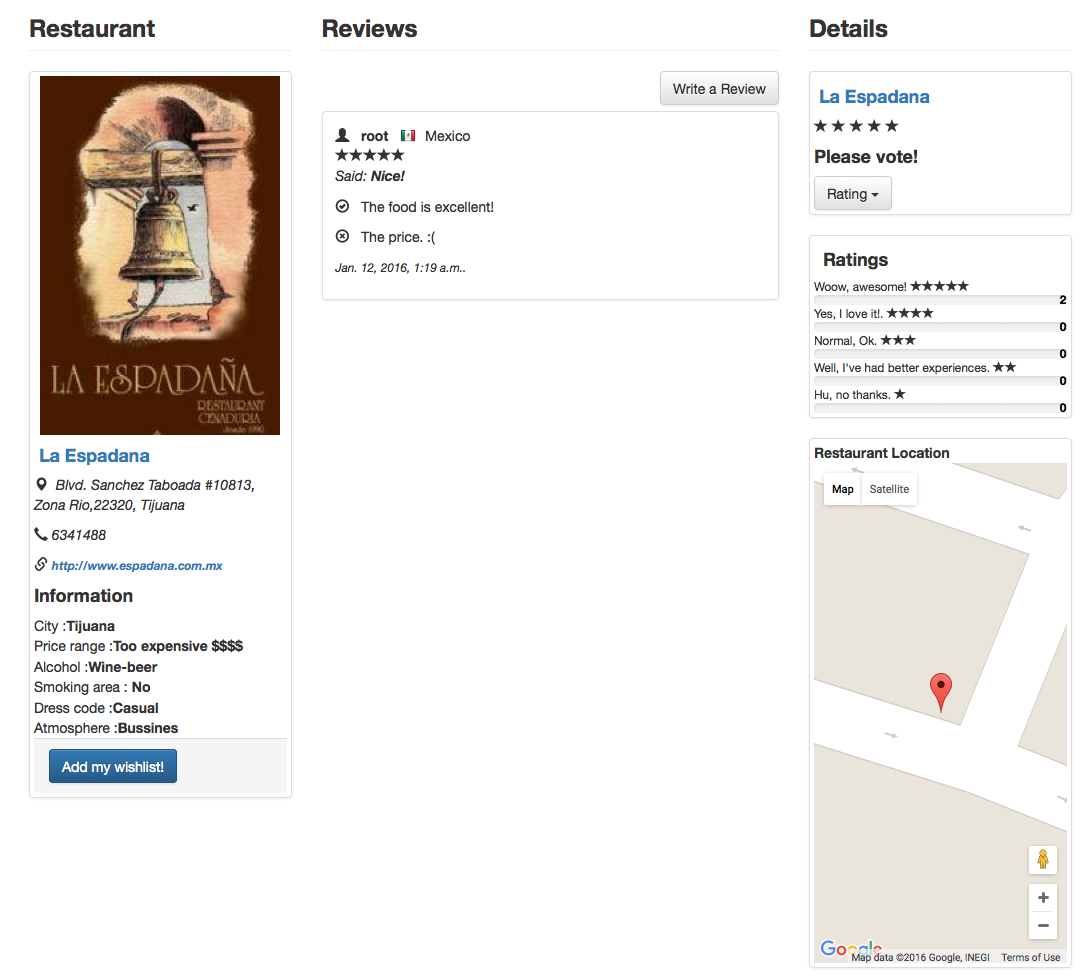
\includegraphics[width=10cm,height=10cm,keepaspectratio]{img/restaurant-model.png}}
\caption{User interface of the restaurant model.}
\label{fig:restaurantmodel}       
\end{figure*}


\section{Fuzzy Logic.}

Fuzzy logic is an approach to computing based on "degrees of truth" rather than
the usual "true or false" (1 or 0) Boolean logic on which the modern computer is
based.  The idea of fuzzy logic was first advanced by Dr. Lotfi Zadeh of the
University of California at Berkeley in the 1960s. Dr. Zadeh was working on the
problem of computer understanding of natural language. Natural language (like
most other activities in life and indeed the universe) is not easily translated
into the absolute terms of 0 and 1. (Whether everything is ultimately
describable in binary terms is a philosophical question worth pursuing, but in
practice much data we might want to feed a computer is in some state in between
and so, frequently, are the results of computing.) It may help to see fuzzy
logic as the way reasoning works, and binary or Boolean logic is simply a
special case of it. Fuzzy logic includes 0 and 1 as extreme cases of truth (or
"the state of matters" or "fact") but also includes the various states of truth
in between so that, for example, the result of a comparison between two things
could be not "tall" or "short" but ".38 of tallness."

Fuzzy logic seems closer to the way our brains work. We aggregate data and
create some partial truths which we aggregate further into higher truths which
in turn when certain thresholds are exceeded, cause certain further results such
as motor reaction. A similar kind of process is used in neural networks, expert
systems, and other artificial intelligence applications. Fuzzy logic is
essential to the development of human-like capabilities for AI, sometimes
referred to as artificial general intelligence: the representation of
generalized human cognitive abilities in software so that, faced with an
unfamiliar task, the AI system could find a solution.

\subsection{Fuzzy inference system.} 

A fuzzy inference system (FIS) is a system that uses fuzzy set theory to map
inputs (features in the case of fuzzy classification) to outputs (classes in the
event of fuzzy classification).  An example of a Mamdani inference system is
shown in Figure x To compute the output of this FIS given the inputs; one must
go through six steps:

\begin{enumerate}
\item  \textbf{Determining a set of fuzzy rules.}
\item  \textbf{fuzzifying the inputs using the input membership functions.} 
\item  \textbf{Combining the fuzzified inputs according to the fuzzy rules to establish a rule strength.} 
\item  \textbf{Combining the fuzzified inputs according to the fuzzy rules to establish a rule strength.} 
\item  \textbf{Combining the consequences to get an output distribution.}
\item  \textbf{Defuzzifying the output distribution (this step is only if a crisp production (class) is needed).}
\end{enumerate}

The following is a more detailed description of this process.

\subsection{Creating fuzzy rules.} 

Fuzzy rules are a collection of linguistic
statements that describe how the FIS should make a decision regarding
classifying an input or controlling an output. Fuzzy rules are always written in
the following form: if (input1 is membership function1) and/or (input2 is
membership function2) and/or . then (output is output membership function). For
example, one could make up a rule that says: if temperature is high and humidity
is high then room is hot. There would have to be membership functions that
define what we mean by high temperature (input1), high humidity (input2) and a
hot room (output1). This process of taking an input such as temperature and
processing it through a membership function to determine what we mean by "high"
temperature is called fuzzification and is discussed in section 3.1.2. Also, we
must define what we mean by "and" / "or" in the fuzzy rule. This is called fuzzy
combination and is discussed in section 3.1.3.

\subsection{Fuzzification.}

The purpose of fuzzification is to map the inputs from a set of sensors (or
features of those sensors such as amplitude or spectrum) to values from 0 to 1
using a set of input membership functions. In the example shown in figure \ref{fig:mamdaniFis},
there are two inputs, x0, and y0 is shown in the lower left corner.These inputs
are mapped into fuzzy numbers by drawing a line up from the inputs to the input
membership functions above and marking the intersection point. 

\begin{figure*}
\captionsetup{justification=centering,margin=2cm}
\centering
\setlength\fboxsep{0pt}
\setlength\fboxrule{0.7pt}
\fbox{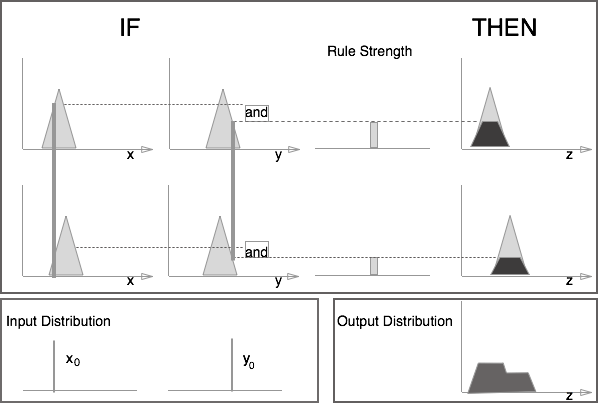
\includegraphics[width=10cm,height=10cm,keepaspectratio]{img/inference-sample.png}}
\caption{A two input, two rule Mamdani FIS with crisp inputs.}
\label{fig:mamdaniFis}       
\end{figure*}

These input membership functions, as discussed previously, can represent fuzzy concepts 
such as "large" or "small", "old" or "young", "hot" or "cold", etc. For example, x0
could be the EMG energy coming from the front of the forearm and y0 could be the
EMG energy coming from the back of the forearm. The membership functions could
then represent "large" amounts of tension coming from a muscle or "small"
amounts of tension. When choosing the input membership functions, the definition
of what we mean by "large" and "small" may be different for each input.

\subsection{Fuzzy combinations (T-norms).} 
In making a fuzzy rule, we use the concept of "and", "or", and sometimes "not". 
The sections below describe the most common definitions of these 
"fuzzy combination" operators. Fuzzy combinations are also referred to as "T-norms".

\subsection{Fuzzy "and"}

The fuzzy "and" is written as: 

\begin{equation}\label{eq:prediction}
\displaystyle \mu_A\cap \mu_B = T(\mu_A(x),\mu_ B(x))  
\end{equation}

where µA is read as "the membership in class A" and µB is read as "the
membership in class B". There are many ways to compute "and". The two most
common are: 

\begin{enumerate}
\item Zadeh - $min(\mu_A(x), \mu_B(x))$.  This technique, named after the
inventor of fuzzy set theory simply computes the "and" by taking the minimum of
the two (or more) membership values. This is the most common definition of the
fuzzy "and". 
\item Product - $\mu_A(x) + \mu_B(x)) - \mu_A(x) \mu_B(x))$.  This technique uses the
difference between the sum of the two (or more) membership values and the
product of the membership values.
\end{enumerate}

Both techniques have the following properties:
\begin{itemize}
\item $T(a,0) = T(0,a) = a$ 
\item $T(a,1) = T(1,a) = 1$
\end{itemize} 
Similar to the fuzzy "and", both
definitions of the fuzzy "or" also can be used to compute the Boolean "or".
Table \ref{tab:boolean_or} shows the Boolean "or" operation. Notice that both fuzzy "or" definitions
also work for these numbers. The fuzzy "or" is an extension of the Boolean "or"
to numbers that are not just 0 or 1, but between 0 and 1.

\begin{table}
\small
\caption{The Boolean "or".}
\label{tab:boolean_or} 
\centering
\small
\begin{tabular}{p{3cm} p{3cm} p{3cm} }
\hline\noalign{\smallskip}
 Input 1 & Input 2 & Input 3 \\
\noalign{\smallskip}\hline\noalign{\smallskip}
\small{0} & \small{0} & \small{0}\\ \hline  
\small{0} & \small{1} & \small{1}\\ \hline  
\small{1} & \small{0} & \small{1}\\ \hline  
\small{1} & \small{1} & \small{1}\\ \hline  
\noalign{\smallskip}\hline
\end{tabular}
\end{table}

\subsection{Fuzzy "and"}

The consequence of a fuzzy rule is computed using two steps: 1. Computing the
rule strength by combining the fuzzified inputs using the fuzzy combination
process discussed in section 4.1.3. This is shown in Figure 4-1. Notice in this
example, the fuzzy "and" is used to combine the membership functions to compute
the rule strength. 2. Clipping the output membership function at the rule
strength. Once again, refer to Figure 4-1 to see how this is done for a two
input, two rule Mamdani FIS.

\subsection{Combining Outputs into an Output Distribution} 
The outputs of all of
the fuzzy rules must now be combined to obtain one fuzzy output distribution.
This is usually, but not always, done by using the fuzzy "or". Figure 4-1 shows
an example of this. The output membership functions on the right-hand side of
the figure are combined using the fuzzy "or" to obtain the output distribution
shown in the lower right corner of the figure.

\subsection{Defuzzification of Output Distribution} 

In many instances, it is desired to come up with a single crisp output from a
FIS. For example, if one was trying to classify a letter drawn by hand on a
drawing tablet, ultimately the FIS would have to come up with a crisp number to
tell the computer which letter was drawn. This crisp number is obtained in a
process known as defuzzification. There are two common techniques for
defuzzifying:

\begin{enumerate} 
\item   Center of mass - This technique takes the output
distribution found in section 4.1.5 and finds its center of mass to come up with
one crisp number. This is computed as follows:
\begin{equation}\label{eq:centerM}
\displaystyle z=\frac{\sum_{j=1}^qz_j\mu_c(z_j)}{\sum_{j=1}^q\mu_c(z_j)}  
\end{equation}

where z is the center of mass and uc is the membership in class c at value zj.
An example outcome of this computation is shown in Figure 4-2.


Falta agregar imagen al path
\begin{figure*}
\captionsetup{justification=centering,margin=2cm}
\centering
\setlength\fboxsep{0pt}
\setlength\fboxrule{0.7pt}
\fbox{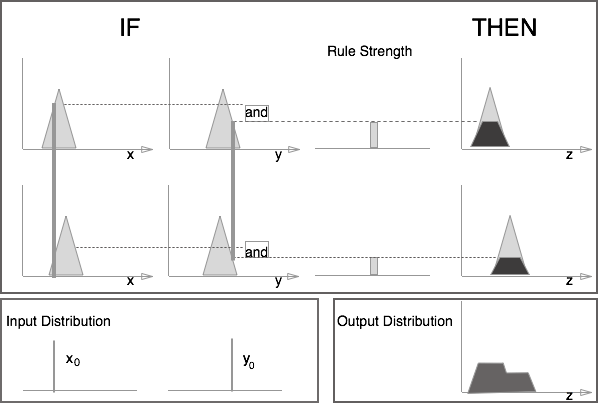
\includegraphics[width=10cm,height=10cm,keepaspectratio]{img/inference-sample.png}}
\caption{Defuzzification Using the Center of Mass.}
\label{fig:centerMass}       
\end{figure*}



\item Mean of maximum - This technique takes the output distribution found in section
4.1.5 and finds its mean of maxima to come up with one crisp number. This is
computed as follows:
\begin{equation}\label{eq:centerM}
\displaystyle z=\frac{\sum_{j=1}^lz_j}{l}
\end{equation}

where z is the mean of maximum, zj is the point at which the membership function
is maximum, and l is the number of times the output distribution reaches the
maximum level. An example outcome of this computation is shown in Figure x.

Falta agregar imagen al path
\begin{figure*}
\captionsetup{justification=centering,margin=2cm}
\centering
\setlength\fboxsep{0pt}
\setlength\fboxrule{0.7pt}
\fbox{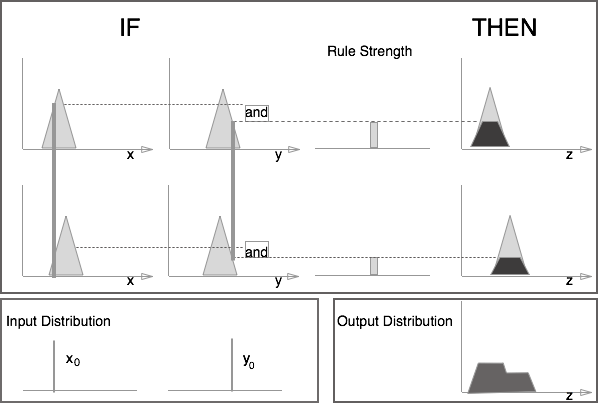
\includegraphics[width=10cm,height=10cm,keepaspectratio]{img/inference-sample.png}}
\caption{Defuzzification Using the Mean of Maximum.}
\label{fig:mean}       
\end{figure*}

\end{enumerate}

\subsection{Fuzzy Inputs.}  
In summary, Figure x-1 shows a two input Mamdani FIS
with two rules. It fuzzifies the two inputs by finding the intersection of the
crisp input value with the input membership function. It uses the minimum
operator to compute the fuzzy "and" for combining the two fuzzified inputs to
obtain a rule strength. It clips the output membership function at the rule
strength. Finally, it uses the maximum operator to compute the fuzzy "or" for
combining the outputs of the two rules. Figure x-4 shows a modification of the
Mamdani FIS where the input y0 is fuzzy, not crisp. This can be used to model
inaccuracies in the measurement. For example, we may be measuring the output of
a pressure sensor. Even with the exact same pressure applied, the sensor is
measured to have slightly different voltages. The fuzzy input membership
function models this uncertainty. The input fuzzy function is combined with the
rule input membership function by using the fuzzy "and" as shown in Figure x-4.

falta agregar el path de la imgen

\begin{figure*}
\captionsetup{justification=centering,margin=2cm}
\centering
\setlength\fboxsep{0pt}
\setlength\fboxrule{0.7pt}
\fbox{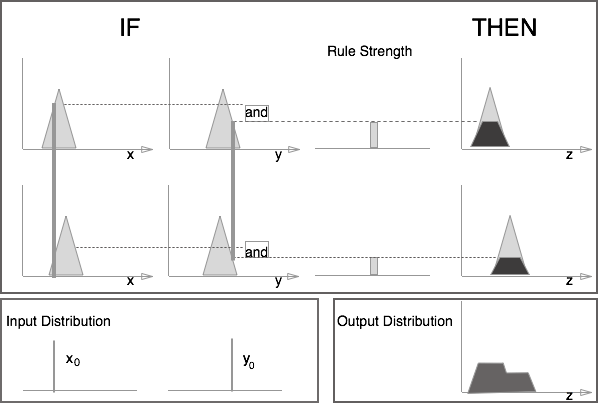
\includegraphics[width=10cm,height=10cm,keepaspectratio]{img/inference-sample.png}}
\caption{A two Input, two rule Mamdani FIS with a fuzzy output.}
\label{fig:fuzzyOut}       
\end{figure*}


\section{Gamification.}

A definition given by  referencia is  “Gamification is the process by which
concepts are brought to the real world task associated with real people”. Also
gamification handle game design elements which are commonly known as non-game
context in the presud to  enhance user engagement, organizational productivity,
flow, learning, evaluations, among others.

\subsection{Techniques.}   
Techniques in this context seek to influence humans
natural desires for competing, learning, mastery,  achievement, status, self-
expression, and socializing[][][][]. Early approaches use rewards for players
who accomplish desired tasks or competition to engage players[]. For instance
some sort of rewards include points,[25] achievement badges or levels,[26] the
filling of a progress bar,[27] or providing the user with virtual currency.[26].
By Making the rewards for  tasks achievements visible to other players or
providing leader boards are ways of encouraging players to compete.[28]. Because
the  problematic consequences of competition, which can result in negative
conduct, low cooperation and collaboration, or disadvantaging certain player
demographics such as women,[29] best-practice gamification designs try to
refrain from using this element.

Another techniques to gamification is to make existing tasks feel more like
games.[30] Some techniques used in this approach include adding meaningful
choice, onboarding with a tutorial, increasing challenge,[31] and adding
narrative.[30]

\subsection{EvoSpace-Interactive} EvoSpace-Interactive is an open source
framework focused on Web environments for collaborative interactive evolutionary
applications. This framework defines three main components for each application,
which are: 
\begin{itemize} 
\item Individual.  
\item Processing Script. 
\item Worker Script. 
\end{itemize}

The individual is represented internally as a data dictionary stored in Redis
[16] database management system; the individual contains main attributes as id,
chro-mosome, mom, dad, and views. This attributes represents the key information
of the individual as the individual offspring, the number of times that the
individual has been selected, etcetera, as we can see in figure \ref{fig:individualRep} [3].

\begin{figure*}
\captionsetup{justification=centering,margin=2cm}
\centering
\setlength\fboxsep{0pt}
\setlength\fboxrule{0.7pt}
\fbox{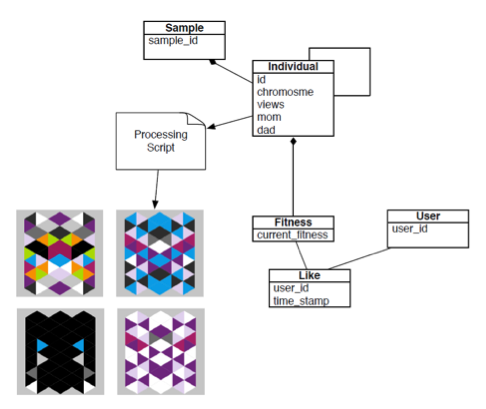
\includegraphics[width=10cm,height=10cm,keepaspectratio]{img/individualRep.png}}
\caption{Individual Representation.}
\label{fig:individualRep}       
\end{figure*}

As we can observe on figure \ref{fig:ESFramework}, this work uses database management systems to
implement collaborative interactive evolutionary applications. One of the
reasons that this framework is using Redis[15] is because it provides a hash-
based imple-mentation of sets and queues, which are natural data structures for
the EvoSpace model. On the other hand this framework uses a relational database
to save basic information about the user extracted from the social platform
(Facebook) through open graph API and OAuth2 authentication.

\begin{figure*}
\captionsetup{justification=centering,margin=2cm}
\centering
\setlength\fboxsep{0pt}
\setlength\fboxrule{0.7pt}
\fbox{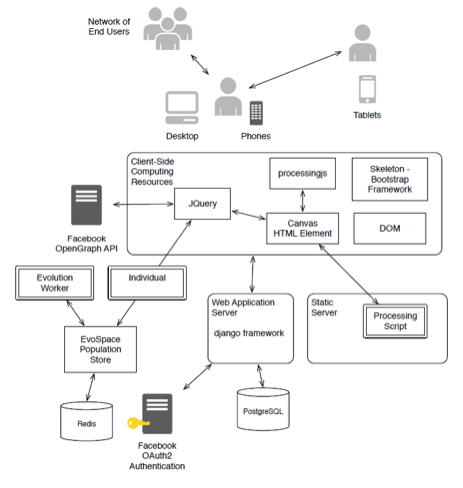
\includegraphics[width=10cm,height=10cm,keepaspectratio]{img/ESFramework.png}}
\caption{EvoSpace-Interactive Framework.}
\label{fig:ESFramework}       
\end{figure*}
